\documentclass[12pt, letterpaper]{article}
\usepackage[utf8]{inputenc}
\usepackage[a4paper, total={7in, 10in}]{geometry}
\usepackage{amsmath}
\usepackage{tikz}
\usepackage{pgfplots}

\title{HW 3}
\author{Ben Lirio}
\date{March 8}

\begin{document}
\maketitle
\begin{enumerate}
	\item Flight
		\begin{enumerate}
			\item In order for a flight with $s = 50$ seats to accomadate $k$ passengers who show up, $k \le s$. Let X represent the random variable of the number of passengers who show up, then $P(X \le s)$ is probability all $k$ passengers will have a seat. This can be calculated as follows, $P(X \le 50) = \rho(45) + \rho(46) + \rho(47) + \rho(48) + \rho(49) + \rho(50) = .05 + .1 + .12 + .14 + .25 + .17 = .83$. There is an \textbf{83\%} chance all ticketed passengers who show up will have a seat.
			\item The probability at least one of $k$ passengers who show up will not be seated happens when $k > s$. Which can be shown as $P(X < 50)$ which is the complement to answer 'a'. so $P(X < 50) = 1 - P(X \le 50) = 1 - .83 = .17$. The probability that not all of the $k$ will recieve a seat is \textbf{17\%}.
			\item If you are the first person on standby, then if there must be one free seat on the plane for you to have a seat. This happens when $X \le 49$. So answer derived from a $P(X < 50) = P(X \le 50) - P(X = 50) = .83 - .17 = .66$. If you are the first person on standby there is a \textbf{66\%} you will still be able to fly. Now, if you are the 3rd person on standby $X \le 47$ must be true. $P(X \le 47) = P(45) + P(46) + P(47) = .05 + .10 + .12 = .27$. If you are the third person on standby there is a \textbf{27\%} chance you will still be able to fly.
		\end{enumerate}
	\item Earthquake
		\begin{enumerate}
			\item The probability distrabution of $X$ is \[ \rho(k) = \begin{cases}
			{4\choose k}.25^k.75^{N-k} & 0 \le k \le 4 \\
			0 & otherwise
			\end{cases}
			\]
			\item 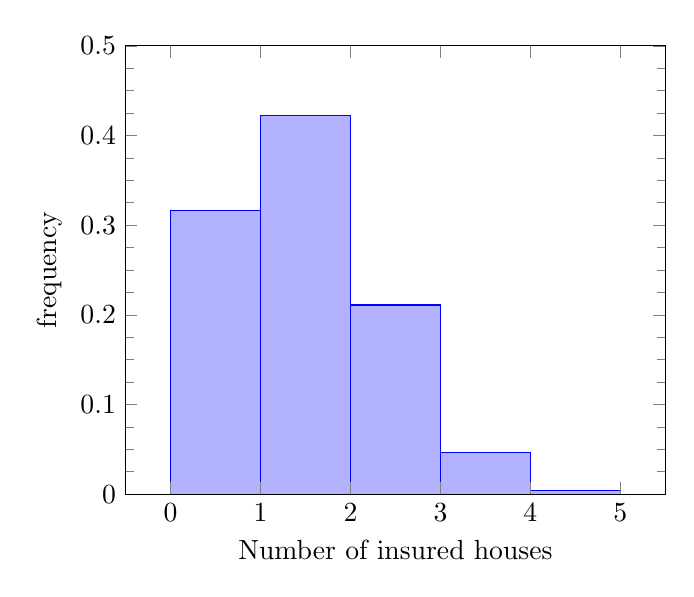
\begin{tikzpicture}
			\begin{axis}[
			ymin=0, ymax=.5,
			minor y tick num = 3,
			area style,
			xlabel={Number of insured houses},
			ylabel={frequency}
			]
			\addplot+[ybar interval,mark=no] plot coordinates {
			(0,.316406)
			(1,.421875)
			(2,0.210938)
			(3,0.046875)
			(4,0.003906)
			(5,0)
			};
			\end{axis}
			\end{tikzpicture}
			\item Initialy I thought of calculating the expected value, $E(X) = \rho n = 1.0$, but then I interpreted the question as the mode, which value individually is most likely to be choosen, which also is \textbf{1}.
			\item The probability at least two of the four selected houses have eathquake insurance can be represented as follows, $P(X \ge 2) = 1 - P(X < 2) = 1 - P(X=0) - P(X=1) = 1 - .316406 - .421875 = 0.261719$. The probability that at least two of the selected houses have earthquake insurance is \textbf{26.1719\%}.
		\end{enumerate}
	\item Allergies
		\begin{enumerate}
			\item one
		\end{enumerate}
\end{enumerate}
\end{document}
